% Results Part Four: Shifting experiments for prediction of better catalysts

\subsection{Shifting experiments for prediction of better catalysts}

% Figure 5: Shifting Experiments
\begin{figure}[htbp]
    \centering
    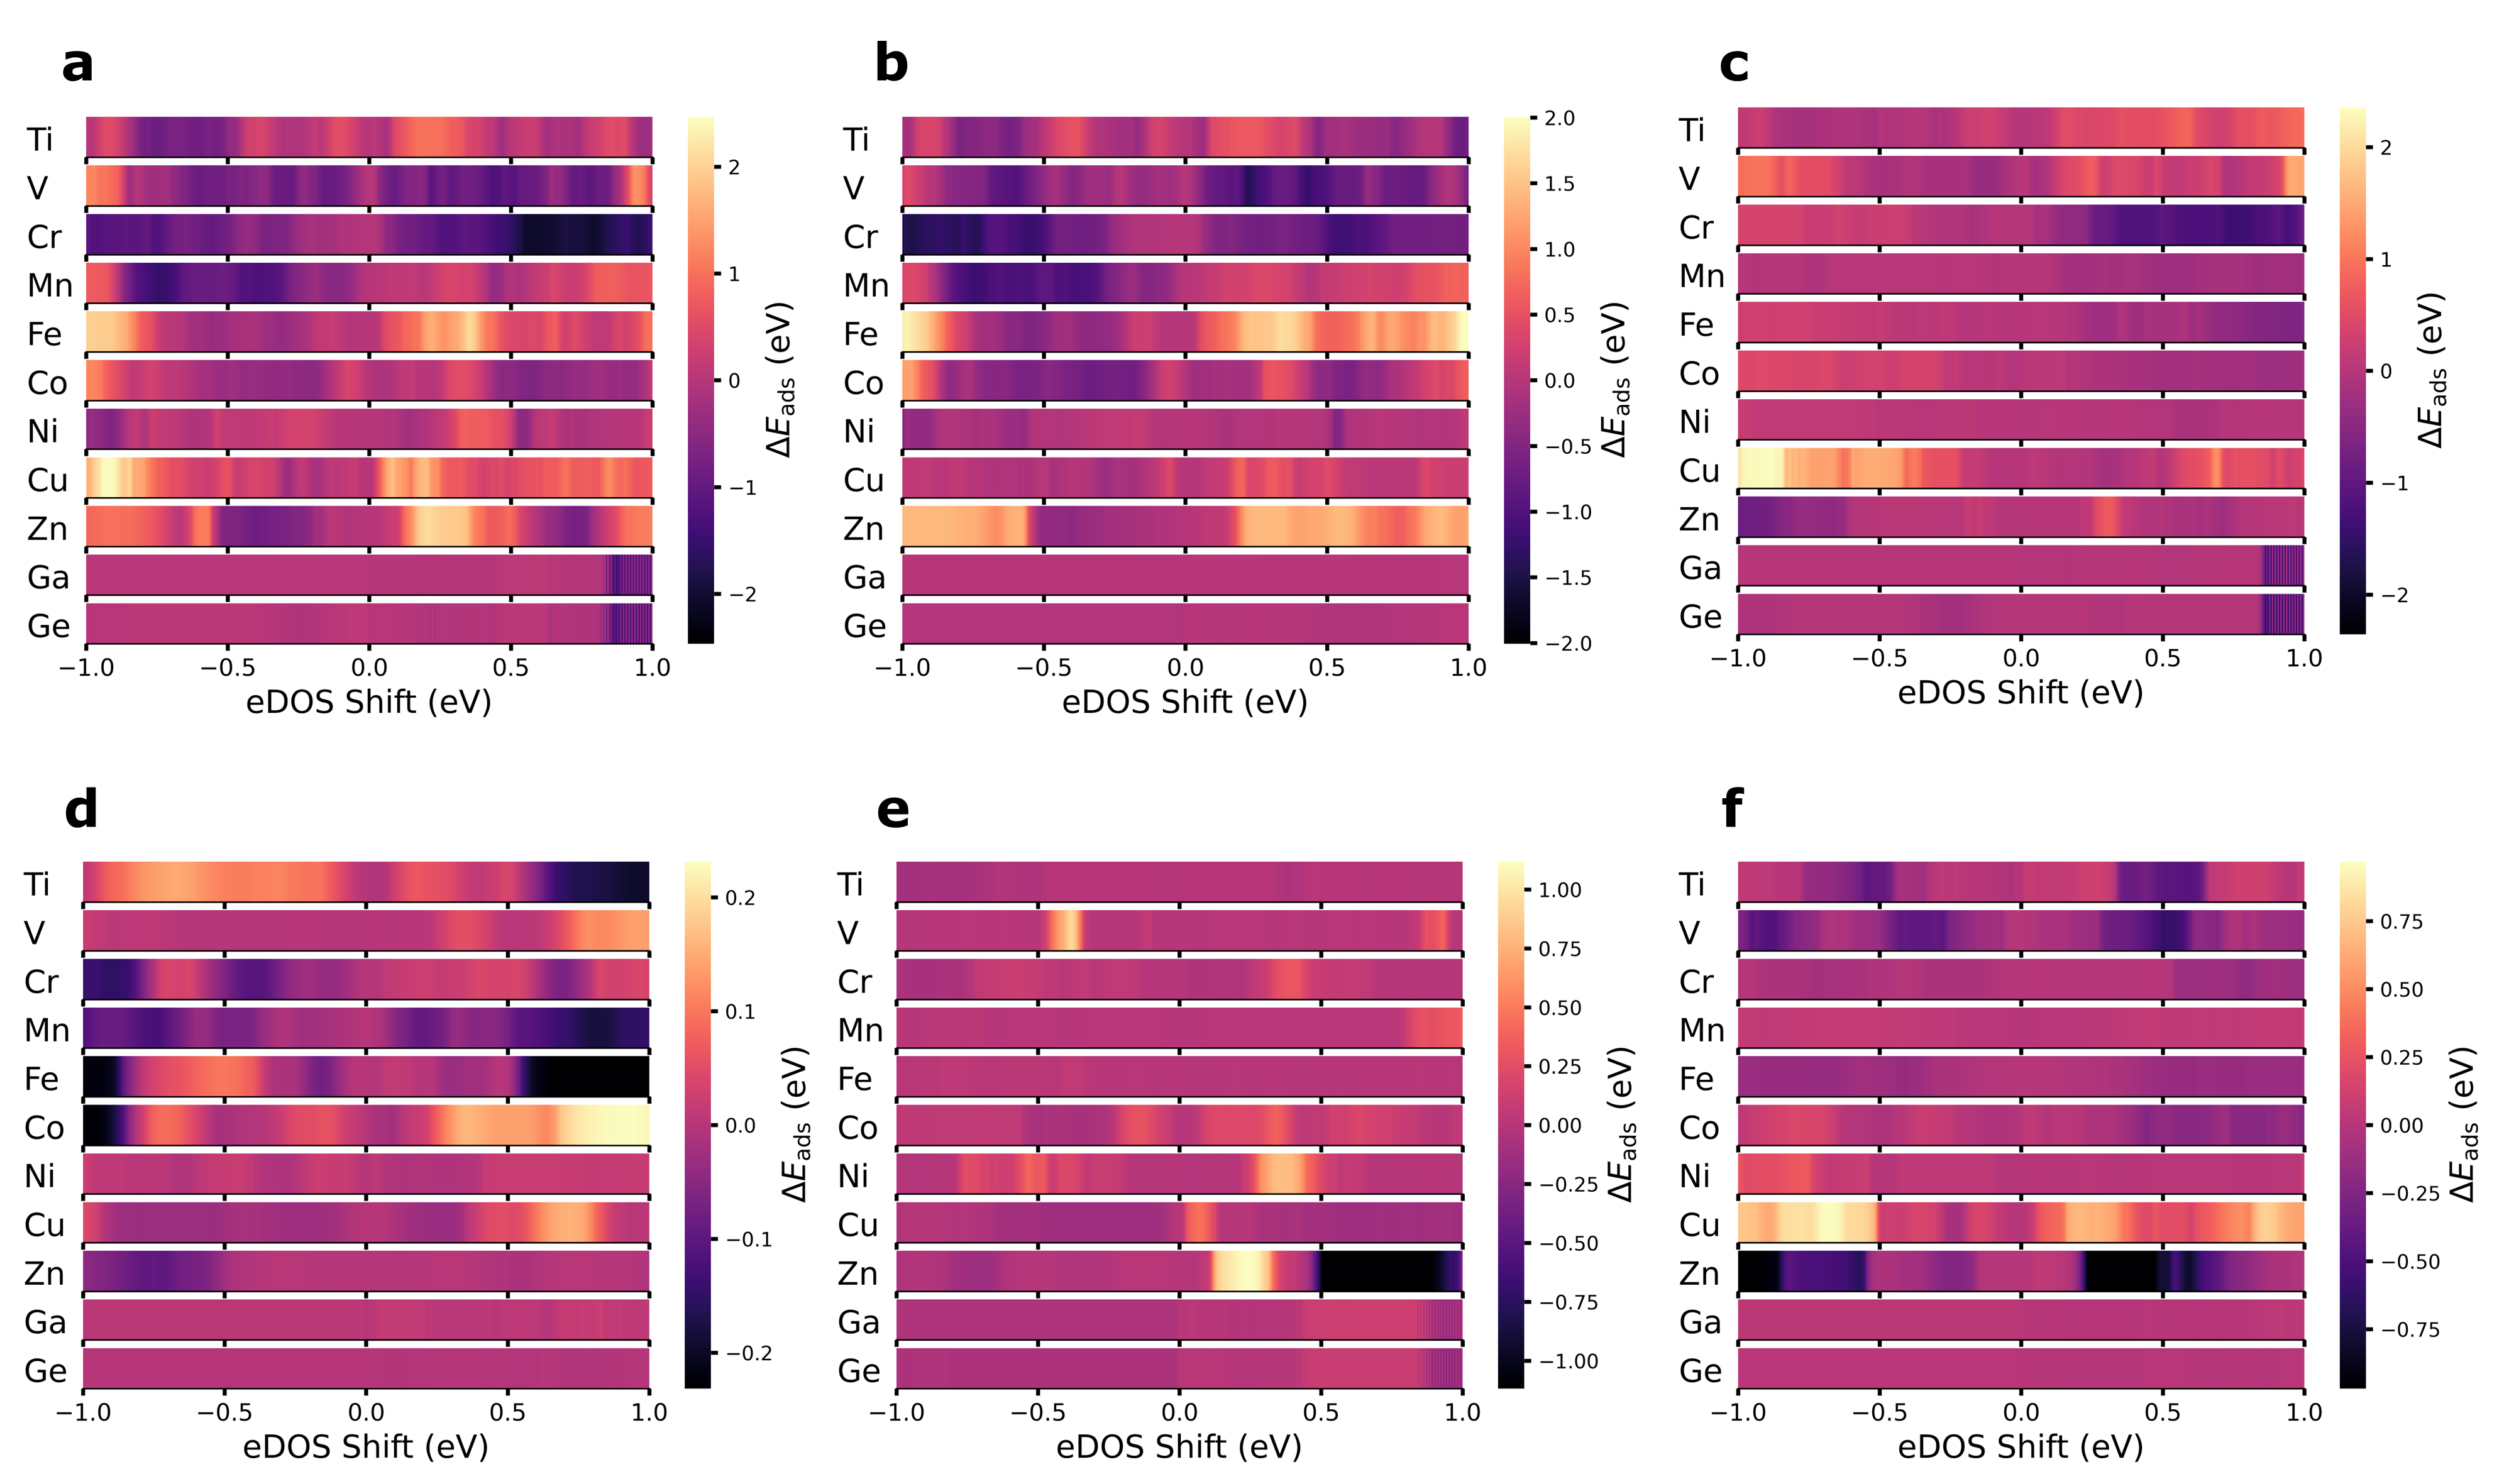
\includegraphics[width=\textwidth]{main_fig5_shifting.png}
    \caption{\textbf{Shifting Experiments.}
    Impact of orbitalwise eDOS shifting on CO adsorption energy, as predicted by the CNN model,
    for single metal atom catalysts supported on g-C\textsubscript{3}N\textsubscript{4}.
    The disturbances caused by shifting of (\textbf{a})entire $d$, (\textbf{b})$d_{xy}$,
    (\textbf{c})$d_{yz}$, (\textbf{d})$d_{z^2}$, (\textbf{e})$d_{xz}$ and
    (\textbf{f})$d_{x^2-y^2}$ orbitals are illustrated.
    The shifting step size corresponds to the energy resolution of the eDOS,
    which is 0.005 eV in this study.
    A positive eDOS shift indicates a shift towards higher energy levels, and vice versa.}
    \label{main_fig5:shifting}
\end{figure}

While CNN models excel in prediction of the activity of catalyst candidates directly from eDOS,
volcano plots point out directions leading to better catalysts.
Exploring potential disturbances to adsorption energies and aiming to shift existing catalyst
candidates closer to the peak of the activity volcano plot presents an intriguing avenue of investigation.
In this work, we introduce an orbitalwise shifting experiment to explore
the impact of orbitalwise eDOS shifting on adsorption behavior.
The experiment involved shifting eDOS along the energy axis,
and the CNN model was deployed to predict the resultant disturbance in adsorption energy for each shifting operation.
Focusing on all Period 4 metal elements examined in this study, we analyzed the effects of eDOS shifting.
To induce a moderate disturbance, we selected the energy range of -1 to 1 eV,
and a shifting resolution of 0.005 eV/step was chosen to align with the eDOS calculation resolution.

\cref{main_fig5:shifting} illustrates that supported Ga and Ge, the sole p-block metals in our study,
exhibited no response to d orbital shifting.
This observation is consistent with their lack of d-electrons in their valence shells,
reinforcing the reliability of our shifting experiments.
We also investigated potential disturbance from p orbital shifting,
as shown in Supplementary \cref{supp_fig31:p_shifting} and found no significant response.
This implies that Ge@g-C\textsubscript{3}N\textsubscript{4} holds promise as a CO\textsubscript{2}RR electrocatalyst,
given its high activity and resilience to electronic structure disturbances.
Nevertheless, fine-tuning its performance through eDOS modulation might pose a challenge.
In contrast, supported Fe, Cu and Zn display strong sensitivity to eDOS shifting.
Interestingly, the adsorption energy consistently shifted towards more positive values, indicating a weakening of the catalyst-adsorbate interaction, regardless of the shifting direction within the investigated energy range.
This underscores the intricate interplay between the supported metal atom and the substrate,
emphasizing the necessity of a tool like the CNN model to predict such disturbances.
Supported Cr exhibited a contrary response to eDOS shifting, strengthening the
interaction with the CO adsorbate regardless of the shifting direction.
Supported Ti, V, Co and Ni showed weak response to eDOS shifting,
suggesting the need for alternative methods beyond manipulating their eDOS
to regulate their interactions with CO adsorbate.

In summary, shifting experiments offer a valuable means to predict the potential
disturbances in adsorption behavior resulting from eDOS shifting,
a task that is challenging to accomplish directly within the DFT framework.
However, it's important to note that achieving the predicted shifting
in actual theoretical or experimental scenarios may not be easily accessible.
Skillful manipulation of the electronic structure of catalyst candidates would be required,
presenting a practical challenge.
In contrast to prior studies on bulk metals \cite{fung2021machine},
wherein the adsorption energy exhibits a continuous shift with eDOS variations,
the response of SACs is notably discrete.
These responses manifest as isolated peaks throughout the shifting range,
attributed to the distinctive structure of SACs.
Despite this challenge, having a tool that can predict the potential impact of
eDOS shifting is advantageous for the theoretical design of SACs.
